En el presente TFM, se nos ha proporcionado a los alumnos un archivo de captura de memoria RAM .mem. Por otro lado, se nos ha proporcionado los resúmenes o hash en MD5 y en SHA1 de los archivos tal y como se muestra en la siguiente imagen.

\begin{figure}[htp]
    \centering
    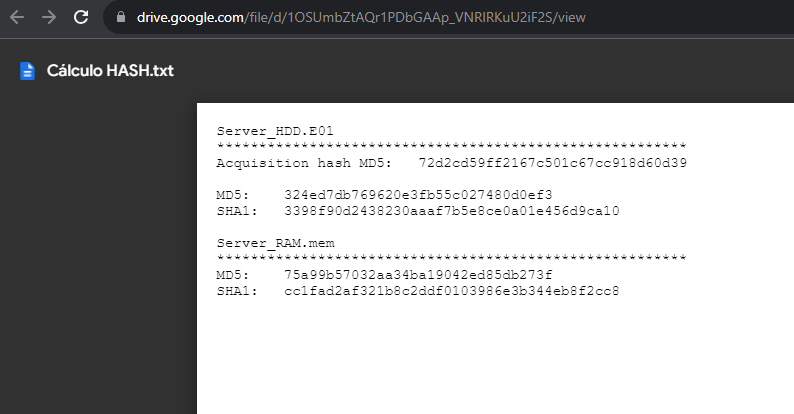
\includegraphics[width=1.0\textwidth]{imagenes/007-imagen-hash-archivos.png}
    \caption{Pantallazo hash imágenes de archivos.}
    \label{Pantallazo hash imágenes de archivos.}
\end{figure}

Como Podemos ver, los hash resúmenes del archivo de la ram, tememos los siguientes hashes en MD5 y en SHA1:

\begin{itemize}
    \item \textbf{MD5:} 75a99b57032aa34ba19042ed85db273f
    \item \textbf{SHA1:} cc1fad2af321b8c2ddf0103986e3b344eb8f2cc8
\end{itemize}

Eñ hash tal y como se indica en los apuntes de la asignatura, en el módulo de Fases y metodología del análisis forense, durante la adquisición de evidencias digitales dice  lo siguiente:

Una vez generada la copia o clon del soporte original, el programa o el dispositivo hardware empleado en este proceso realiza el cálculo del CRC o del valor hash del soporte original y del destino, con la finalidad de garantizar que los dos son idénticos y que la copia se ha producido sin ningún error. Este cálculo puede realizarse sobre todo el conjunto de información contenida en el soporte original, o bien emplear solamente un conjunto de ficheros del total.

A su vez, en el glosario de términos la definición de hash es la siguiente:

Es una función matemática unidireccional que resume un mensaje de tamaño variable (por ejemplo, un archivo), en una representación de tamaño fijo. Es poco probable que dos ficheros distintos tengan la misma representación hash, lo cual significa que este valor puede utilizarse a efectos de comprobación de la integridad de un archivo (o de un sistema entero). Las funciones hash más conocidas son MD5 y SHA-1.

Una vez descargado el archivo de captura de la memoria RAM, procedemos a usar PowerShell para determinar el hash del archivo. Para ello usamos el comando  Get-FileHash [Argumento] -Algorithm MD5. En nuestro caso hemos usado los siguientes comandos:


\begin{verbatim}
Get-FileHash .\Server_RAM.mem -Algorithm MD5
\end{verbatim}


\begin{verbatim}
Get-FileHash .\Server_RAM.mem -Algorithm SHA1
\end{verbatim}



La respuesta de PowerShell es el siguiente respectivamente

\begin{verbatim}
Algorithm       Hash                                                                   Path
---------       ----                                                                   ----
MD5             75A99B57032AA34BA19042ED85DB273F                                       D:\TFM\RAM\...
\end{verbatim}

\begin{verbatim}
Algorithm       Hash                                                                   Path
---------       ----                                                                   ----
SHA1            CC1FAD2AF321B8C2DDF0103986E3B344EB8F2CC8                               D:\TFM\RAM\...
\end{verbatim}

Se puede observar en la siguiente imagen la respuesta de PowerShell de los hashes de MD5 y SHA1.

\begin{figure}[htp]
    \centering
    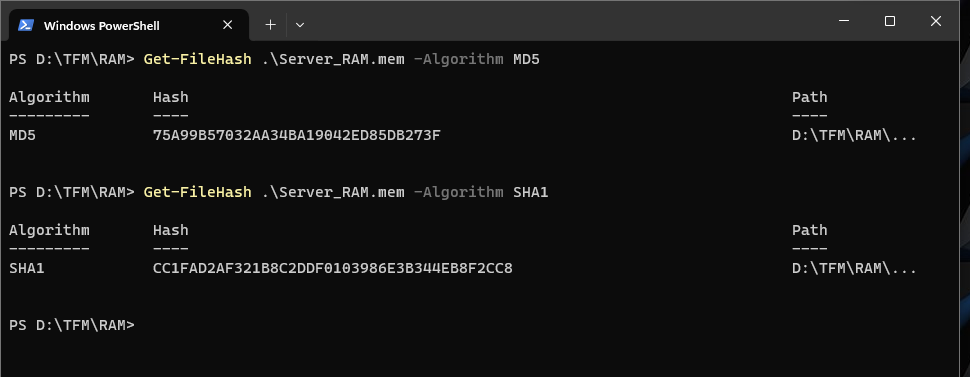
\includegraphics[width=1.0\textwidth]{imagenes/008-captura-hash-PowerShell.png}
    \caption{Hash Ram en PowerShell.}
    \label{Hash Ram en PowerShell.}
\end{figure}

Como conclusión podemos verificar que la integridad de la copia facilitada para realizar el TFM no ha sido vulnerada.